\iffalse
\bibliography{../bib/thesis.bib}
\fi

\chapter{绪论}
随着科技的进步和Internet的迅速普及和不断发展,互联网正密切影响着人们的工作、学习和生活,即时通信、电子邮件、电子商务、在线交易等与人们的日常生活息息相关。2017年1月,中国互联网络信息中心发布了第39次《中国互联网络发展状况统计报告》,截至2016年12月,我国网民规模达到7.31亿,普及率达53.2\%,网民规模已经相当于欧洲人口总量\cite{cnnic2017report}。然而,伴随着信息化快速发展的同时,网络安全形势日益严峻:个人信息可能被木马非法盗取、个人账号和密码也可能被恶意获取、电子邮件含有病毒、即时通信工具传播病毒、网上下载的资源携带病毒、网页被植入木马以及快速兴起的社交平台都成为了黑客们的目标。恶意软件(Malware)伴随着飞速发展的信息技术也在快速的发展,成为了危害网络安全甚至社会安全的一个难题。

恶意软件本质上是各种恶意、侵入性的软件或程序代码,旨在未经用户知情和授权的情况访问计算机系统以安装和执行以达到不正当目的。恶意软件的目的往往是盗取用户的各类私密账号,从而从中获取不法利益,造成了普通用户在财力和人力上的损失。据估计,我国约有高达10\%到20\%的电脑被感染了各种恶意软件,造成的损失达到每年数十亿之多。国家互联网应急中心(CNCERT)发布的《2015年中国互联网网络安全报告》\cite{cncert2016report}指出:2015年,共有1978万个IP地址的主机被植入木马或僵尸程序;6.4万个服务器被境外的木马控制;移动互联网恶意程序数量近148万个,较2014年增长了55.3\%;针对境内网站的仿冒页面数量达18万余个,较2014年增长了85.7\%,其中83.2\%的仿冒网站位于境外;工业控制系统也面临着严峻的网络安全威胁。

恶意软件已经成为影响世界各个方面的全球性问题。根据微软发布的安全情报报告,大部分的网络安全威胁均来自于恶意软件。随着影子互联网经济的兴起,恶意软件已不再是单纯用来损坏、破坏或闯入计算机网络系统,但现在主要被用黑客和犯罪分子用来谋取私利。全球在线犯罪的数量已经超过了毒品交易。由于经济利益的驱使,恶意软件呈现爆炸式的增长,现有安全厂商检测和分析能力已经达到极限。海量的新型恶意软件和日益庞大的恶意软件特征库大大增加了安全专家分析和检测的难度。传统安全软件通过特征码比对进行恶意软件查杀、拦截的方式已经远远不能满足新的网络安全态势。

综上所述,有必要研究新型、高效、可靠的方法和技术,实现对恶意软件进行自动化的检测分析,从而保护网络用户的安全。
\section{恶意软件概述}
\subsection{恶意软件定义}
目前恶意软件(Malware, Malicious Software)未有一个统一明确的定义。很多专家学者尝试通过描述其本质特征来对恶意软件做出定义。1986年,Fred Cohen在其博士论文中第一次对计算机病毒进行了定义\cite{cohen1985computer}:病毒是可以通过符号序列来描述,并且能够在合适的环境中通过其自身的拷贝或衍生修改其他的符号序列。1983年,Cohen在VAX11/750系统上展示了类似病毒的程序,该程序能够自行安装或感染其他系统对象,这是实验性计算机病毒的诞生。McGraw和Morrisett\cite{mcgraw2000attacking}将恶意软件定义为``恶意软件是指具有恶意功能的程序,如对计算机系统的安全构成威胁、破坏计算机系统或者在未经计算机用户授权许可的情况下获取计算机系统的敏感信息''。
\subsection{恶意软件分类}
根据使用目的和传播方式的不同,恶意软件通常包括计算机病毒、蠕虫、特洛伊木马、后门、间谍软件、垃圾广告软件等多种类型。
\begin{asparaenum}
\item \textbf{计算机病毒(Virus)}。计算机病毒是最早被提出的恶意软件。早在1949年,冯$\cdot$诺依曼在论文《复杂自动机组织论》\cite{Neumann1966Theory}中勾勒了计算机病毒的蓝图:``一部事实上足够复杂度机器能够复制自身'',当时距离第一台商用计算机问世还有好几年。《中华人民共和国计算机信息系统安全保护条例》中指出:``计算机病毒,是指编制或者在计算机程序中插入的破坏计算机功能或者毁坏数据,影响计算机使用,并能自我复制的一组计算机指令或者程序代码''\cite{gov1994Standard}。从上世纪80年代第一代计算机病毒诞生开始,至今已经发展了数代,代码的复杂程度越来越高、传播速度越来越快、生存能力也越来越强。
\item \textbf{蠕虫(Worm)}。蠕虫是具有自我繁殖能力,可以在无需人工干预的情况下自动利用计算机网络来传播的一种恶意软件\cite{skoudis2004malware}。蠕虫利用多种形式的网络来进行传播,例如电子邮件、即时通信、文件共享(P2P)、局域网和广域网等。蠕虫使用各种漏洞和方式来渗透目标设备并执行代码,这些方式可能包括诱使邮件收件人打开邮件的附件、不当的网络配置、对外公开内部计算机接入权限的网络或者操作系统和应用程序中的漏洞等。最初的蠕虫通常没有破坏功能,仅仅是利用网络进行自身的传播。但是随着网络的发展,蠕虫也开始采用和病毒类似的破坏技术,具备了病毒的可自我复制和传播的特征。
\item \textbf{特洛伊木马(Trojan Horse)}。特洛伊木马(简称木马)是伪装成合法的程序并在用户不知情的情况下隐秘运行来达到非法目的的一种恶意软件,名称来源于希腊神话《特洛伊战争》\cite{trojanhorseWiki}。木马表面上看起是正常的应用程序,实际却能危害计算机安全甚至导致严重破坏。初期的木马仅仅是用来进行非法远程控制的黑客工具,自身并没有传播能力。然而在现在大多数的木马都加入了计算机病毒的功能,从而使得其具有较大的威胁和破坏力。
\item \textbf{后门(Backdoor)}。后门是一种存在于目标系统中,并绕过正常授权流程对目标系统进行远程控制的恶意软件\cite{skoudis2004malware}。当系统被攻破时,一个甚至多个后门程序将被植入到系统中,使得黑客能够轻易的控制目标系统。通常计算机生产厂商在生产计算机时会在系统中植入后门以便为客户提供便捷的技术服务,但是这些后门从未进行可靠性验证。
\item \textbf{Rootkit}。Rootkit是一种持久并毫无察觉地驻留在目标计算机中,长久的维持对系统进行操纵、并通过隐秘渠道收集数据的程序。Rootkit的作用是长时间的保持对目标系统的远程控制。
\item \textbf{间谍软件(Spyware)}。间谍软件是一种在计算机用户不知情的情况下,将用户的私密信息收集并发送给攻击者的程序。间谍软件通常捆绑在正常的软件中,在安装正常软件的同时也安装了间谍软件。
\end{asparaenum}

事实上,目前对恶意软件的分类并不十分明确,在信息技术快速发展的今天,恶意软件的形式多样,功能清大,很多恶意软件都兼有几种类别的恶意行为。随着互联网的快速发展和各类恶意软件技术的快速成熟,新一代的恶意软件已经由过去以制作者炫耀技术为主的个人作品转变为网络罪犯们牟取私利的一种工具。在巨大的利益诱惑面前,进而逐渐发展成为了一个庞大的黑色产业链。

\subsection{恶意软件传播介质}
\subsubsection{网络服务漏洞}
在服务器上运行的网络服务为网络中的客户提供共享的资源和服务。例如,DNS服务提供域名解析服务,文件服务器在网络上提供共享存储。许多商业化的操作系统具有已经安装并运行的各种网络服务。攻击者可以利用此类服务中的漏洞对提供服务的目标机器实施攻击。这类操作系统(例如Microsoft Windows)的大面积安装部署为攻击者利用漏洞植入恶意软件提供了机会。这个特征使网络服务漏洞成为蠕虫感染的首选方法。此外,提供对远程用户使用密码认证进行远程系统访问的服务(例如,SSH)经常暴露于字典攻击,这样的攻击不断地尝试使用存储在字典中的密码登录系统。
\subsubsection{网络下载}
网络下载方式通常以受攻击者的网页浏览器为目标,通过浏览器程序的漏洞,从网络上获取恶意代码并在目标系统上执行。这一过程通常无需与用户进行交互。与网络服务漏洞被动接受感染所不同的是,网络下载是主动的,无法通过防火墙进行防御。目前,常用的攻击技术有API误用和网页浏览器漏洞利用。攻击者可以利用特定的API从网络上下载任一文件,并在目标系统上运行所下载文件。广泛使用的浏览器插件给了攻击者大量的简单可行的攻击方式。
\subsubsection{移动存储}
恶意软件通过自复制将自身文件复制到任何接入到已感染系统的移动存储介质中。在复制的同时,在移动存储中创建autorun.inf文件已保证自身能够自动运行。

\section{恶意软件检测与分析研究进展}
\subsection{特征码匹配技术}
目前,各大安全厂商的反病毒产品主要是基于特征码匹配的。特征码是可执行程序中用作标识的唯一代码片段,通常以字节序列或者指令序列的形式表示。通过反向工程工具反编译可执行文件,信息安全专家人工测试分析反编译得到的代码以选取和确定唯一的特征码。特征码存储在特征码数据库中。基于特征码匹配的恶意软件检测在扫描文件时将搜索特征码数据库进行模式匹配,查找当前文件是否在特征码数据库中有相同或者相似的特征码,若有则判定当前文件为恶意软件,反之则判定为良性。
图\ref{fig:intro:signatureFlow}

\begin{figure}[!ht]
\centering
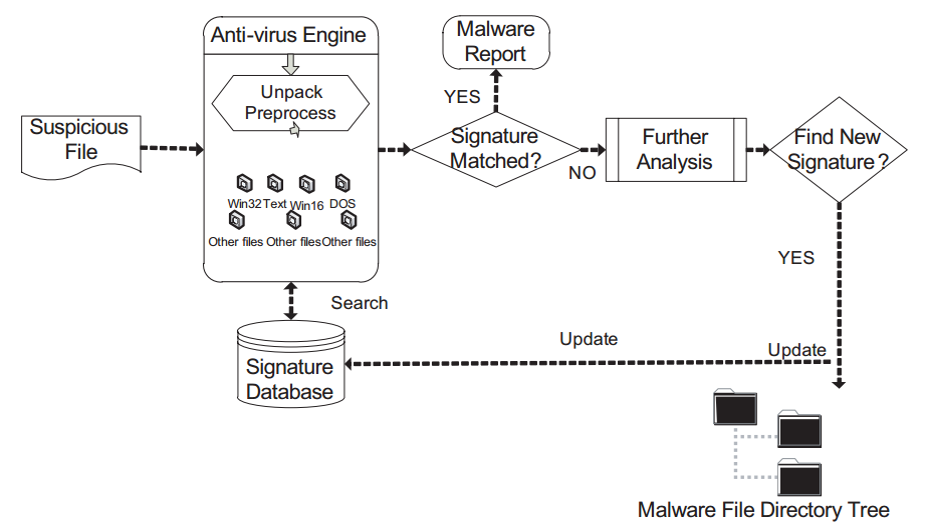
\includegraphics[width=4.5in]{img/intro/signatureFlow.png}
\caption{特征码匹配流程}
\label{fig:intro:signatureFlow}
\end{figure}

\subsection{静态分析与检测技术}
\subsection{动态分析与检测技术}